\documentclass[12pt]{article}

% PACKAGES
\usepackage[utf8]{inputenc}
\usepackage{amsmath}
\usepackage{amssymb}
\usepackage{float}
\usepackage{graphicx}
\usepackage{enumerate}
%\usepackage{mathtools}
\usepackage{hyperref}

% CUSTOM STYLES
%\providecommand{\e}[1]{\ensuremath{\times 10^{#1}}}
%\DeclarePairedDelimiter\abs{\lvert}{\rvert}%

\usepackage{listings}
\usepackage{color}

\definecolor{dkgreen}{rgb}{0,0.6,0}
\definecolor{gray}{rgb}{0.5,0.5,0.5}
\definecolor{mauve}{rgb}{0.58,0,0.82}

\lstset{frame=tb,
  language=Mathematica,
  aboveskip=3mm,
  belowskip=3mm,
  showstringspaces=false,
  columns=flexible,
  basicstyle={\small\ttfamily},
  numbers=none,
  numberstyle=\tiny\color{gray},
  keywordstyle=\color{blue},
  commentstyle=\color{dkgreen},
  stringstyle=\color{mauve},
  breaklines=true,
  breakatwhitespace=true
  tabsize=3
}

\restylefloat{table}

% METADATA
\title{\textbf{FPGA Implementation of the Fast Fourier Transform}}
\date{December 2, 2014}
\author{Garrett Massman and Cory Walker}

\begin{document}

  \maketitle
  \clearpage

  \section*{Introduction}
    In this project we implemented a fast Fourier transform algorithm on a Xilinx FPGA using VHDL. The primary motivation of our project was to digitally analyze musical signals, but the use cases for an FFT chip far surpass that specific use case. \\
    
    As a very general overview, our completed device functions by sampling an analog signal for a set amount of time and storing the data into an input buffer in BRAM. Next, the signal is is processed using an FT controller and a complex ALU and stored in an output buffer. Finally, a microcontroller can then read the output buffer over a standard SPI protocol. From there the processed frequency domain data can be sent to a computer for further processing or any other device.

  \section*{Theory}
    To understand the discrete Fourier transform, one must first analyze its analogous continuous    time form.
    This is written most simply as
    \begin{align*}
    &X(\omega) = \int_{-\infty}^{\infty} x(t) e^{-j \omega t}\,dt
    \end{align*}
    which defines the transform of a continuous time signal $f(t)$.
    Without getting into too many details, it defines the signal as a combination of sinusoids,      making it a very useful tool for real world applications.\\

    The discrete Fourier transform (DFT) is simply a reduction of the continuous Fourier transform   into a discrete sample space.
    In other words, if we let $x_n$ represent a sampled version of the continuous time function      $x(t)$ with a total of $N$ samples, we can replace the integral with a summation over the series, as shown below.
    \begin{align*}
        &X_k = \sum\limits_{n=0}^{N-1} x_n e^{\frac{-j2\pi kn}{N}}
    \end{align*}
    As with the continuous time case, this series gives us a glimpse into the component elements of  our original signal.
    However, it is rather costly to compute, requiring a time complexity of $O(N^2)$.
    For each value $X_k$, a series of values from $n = 0$ to $N - 1$ must be generated and summed,   using up valuable computer resources.
    Thus, calculating the DFT in this way is very inefficient, so we instead turned to the fast  Fourier transform.\\

    In order to perform this operation more quickly, we utilized the Cooley-Tukey FFT algorithm.
    However, the one requirement is that our input is strictly a power of 2.
    That is because the algorithm works by recursively finding the FFT of smaller and smaller sample sizes of $x_n$, which arises from the fact that the transform itself is periodic.
    The transform function can be broken into the sum of its even and odd components,
    \begin{align*}
        &X_k = \sum \limits_{m=0}^{N/2-1} x_{2m}e^{-\frac{2\pi i}{N} (2m)k} + \sum \limits_{m=0}^{N/ 2-1} x_{2m+1} e^{-\frac{2\pi i}{N} (2m+1)k}
    \end{align*}
    This equation can further be simplified by making the substitutions
    \begin{align*}
        &E_k = \sum \limits_{m=0}^{N/2-1} x_{2m}e^{-\frac{2\pi i}{N} (2m)k}
        &O_k = \sum \limits_{m=0}^{N/2-1} x_{2m+1} e^{-\frac{2\pi i}{N/2} mk}
    \end{align*}
    giving us
    \begin{align*}
        &X_k = E_k + e^{-\frac{2\pi i}{N} k} O_k
    \end{align*}
    The expression $e^{-\frac{2\pi i}{N}k}$ is commonly called the \textit{twiddle factor}.
    Furthermore, because of the periodicity of the transform, we can calculate respective even and   odd components simultaneously
    \begin{align*}
        &E_k = E_{k+\frac{N}{2}}
        &O_k = O_{k+\frac{N}{2}}
    \end{align*}
  
  \section*{Stuff That's Already Been Done (change section name plz)}

  \section*{Motivation}

  \section*{System Overview}
    A critical task in building our FFT device was converting an arbitrary waveform into the SPI signal input that the FPGA expected. This requires the use of a fast analog to digital converter. The Xilinx Spartan 3E FPGA does not come with an onboard ADC. Because of this, a large percentage of the work was actually electronics work done outside of the FPGA:

    \begin{figure}[H]
      \centering
      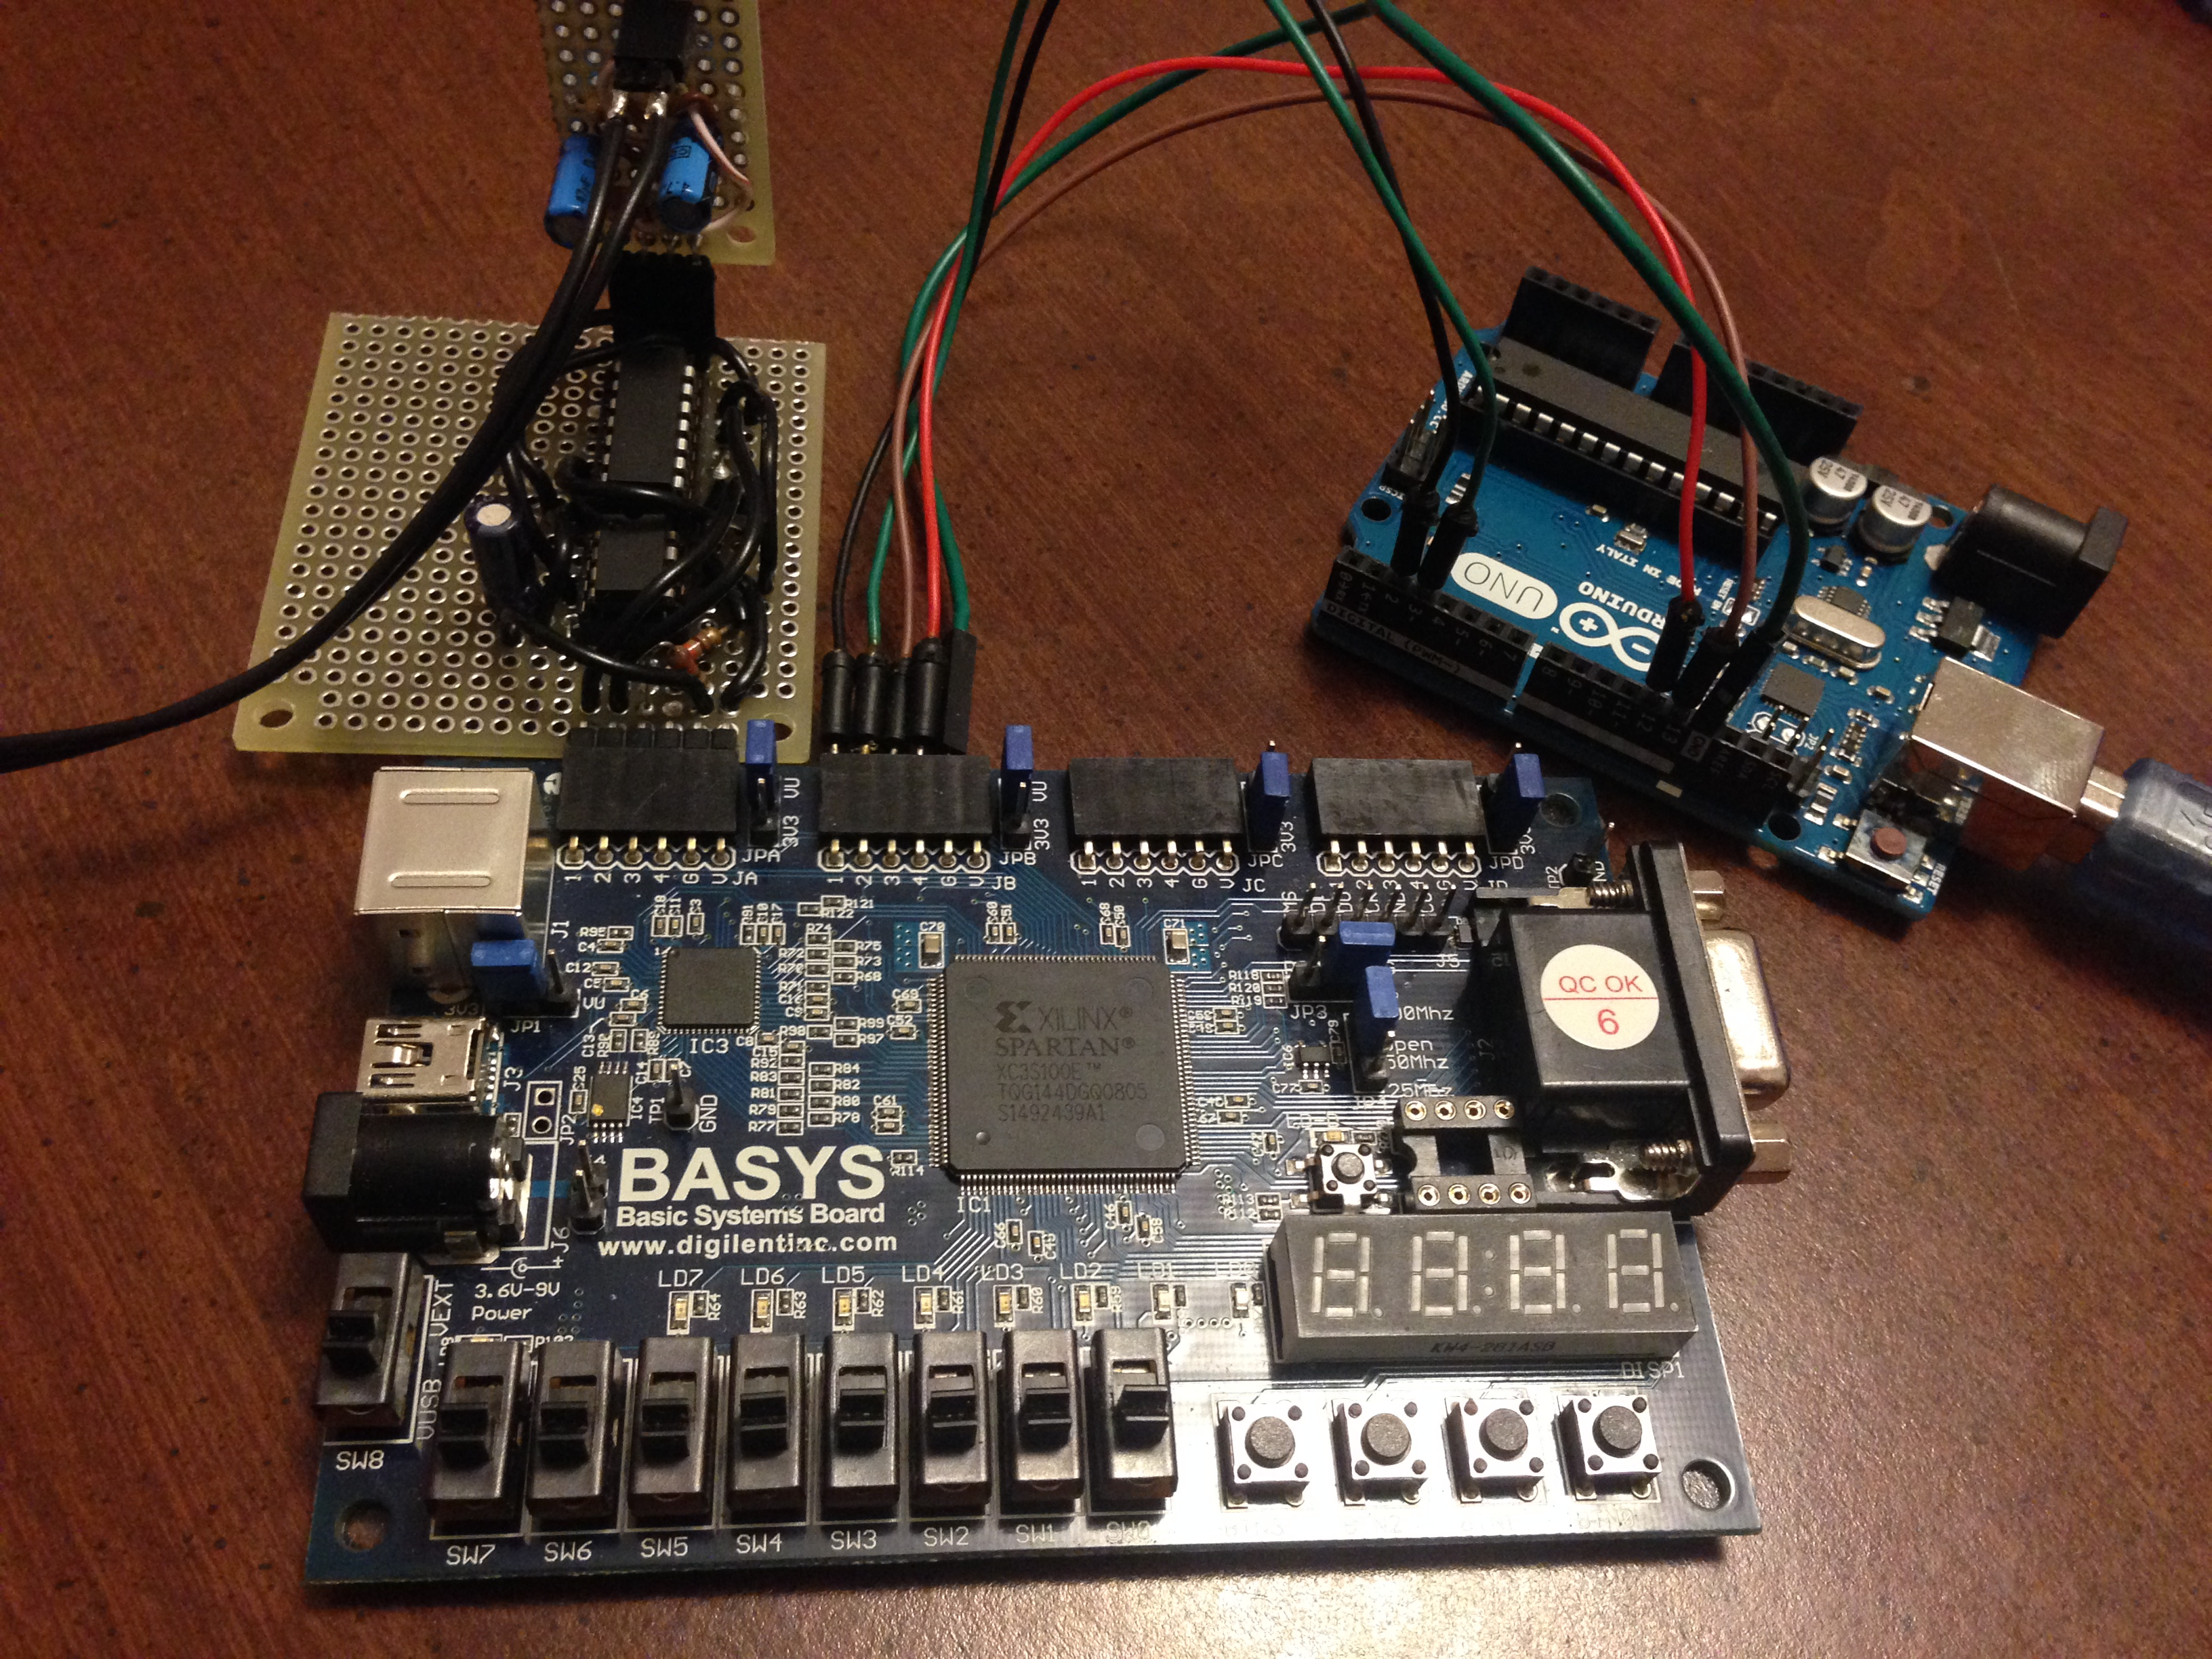
\includegraphics[width=100mm]{full_system.JPG}
      \caption{Full system including ADC PMOD and audio signal module.}
      \label{overflow}
    \end{figure}
    
    These external components condition the signal and then send the digital signal into the FPGA at the right voltage level. In addition, the FPGA's output buffer must be read out by an Arduino microcrontroller and sent to a computer with the right software to parse and display the output. We call these external components macro-components and we call the FPGA internal blocks micro-components.
  
  \section*{Macro-Component Descriptions}
    The required components external to the FPGA are as follows:
    \subsection*{Audio signal module}
      \begin{figure}[H]
        \centering
        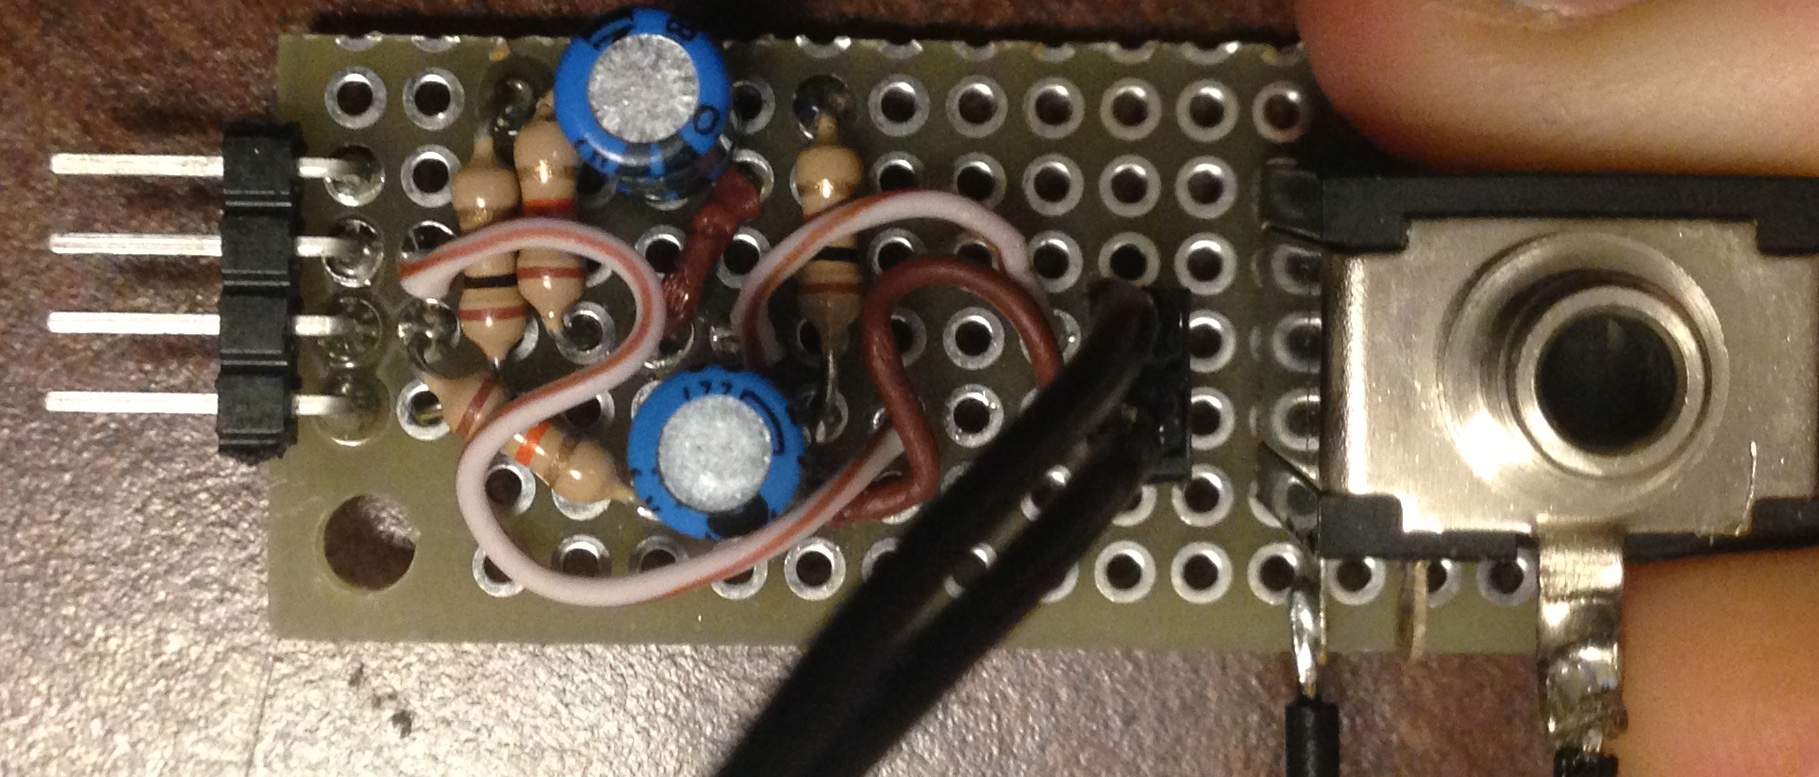
\includegraphics[width=60mm]{audio_sig_mod.JPG}
        \caption{Audio signal circuit board with audio connector}
        \label{overflow}
      \end{figure}
      The audio signal module tailors the input audio signal for conversion with the ADC. Traditional audio signals are centered around 0 V and are in the negative voltage range half the time. This module biases the signal by 2.5 V, allowing for a 5 V variation peak to peak in the audio signal without any clipping. This module also provides filtering capacitors that remove most of the supply rail noise that may be present.

    \subsection*{ADC PMOD}
      \begin{figure}[H]
        \centering
        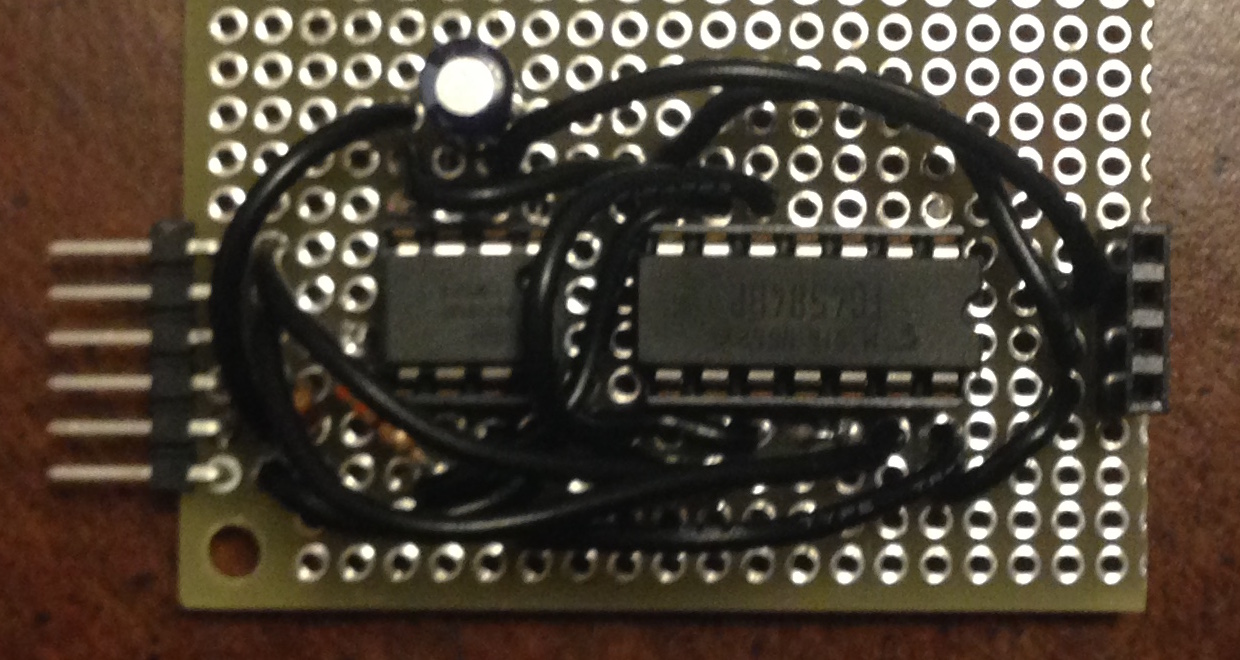
\includegraphics[width=75mm]{adc_pmod.JPG}
        \caption{ADC PMOD circuit board}
        \label{overflow}
      \end{figure}
      The ADC PMOD accepts any input analog input and converts it to a SPI bus that the FPGA can read. The analog signal is fed into the onboard ADS7818 chip. Unfortunately, this chip operates at 5 V but the FPGA operates at 3.3 V. Because of this, there is a voltage divider to drop the voltage down to the FPGA. For FPGA output to be read by the ADS7818, we added a Schmitt inverter IC wired as a Schmitt trigger to act as a level converter.
      \begin{figure}[H]
        \centering
        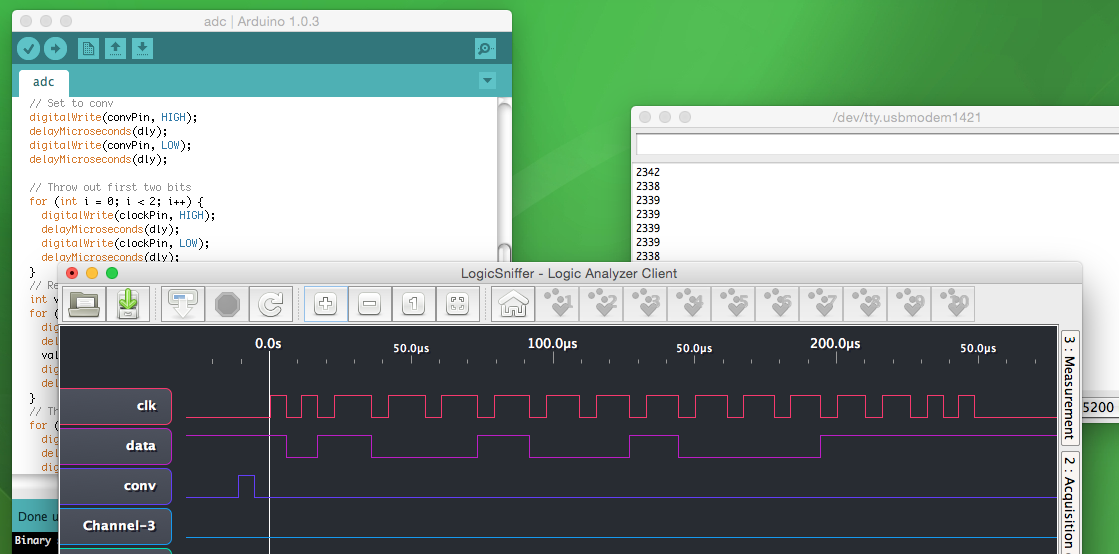
\includegraphics[width=100mm]{adc_logic.png}
        \caption{ADC interfacing}
        \label{overflow}
      \end{figure}
      We started interfacing with the ADS7818 using an Arduino. Once we understood the protocol completely, we moved the interfacing code from the Arduino to the FPGA and started using real signal data.

    \subsection*{Arduino}
      The Arduino functions as a means of getting the processed information out of the FPGA's BRAM. The Arduino turned out to be the main bottleneck in terms of framerate to the computer's display. We had to push the SPI and serial write functions outside of recommended bounds to get a fluid framerate on the computer display. The full software is available in the \texttt{arduino/osc\_binary\_spi} directory of the source code repository.

    \subsection*{Computer software}
      The computer software for this project is divided into two components. The first component is the Python module that facilitates the reading and decoding of the data from the serial port. It will read out 512 complex numbers and, optionally, compute the magnitude of each of those numbers. The second component is the actual display. It will use the Python module to read the device and it uses Tkinter to display the plot on the screen.

  \section*{Micro-Component Descriptions}
    The final block diagram of our device is as follows:
    \begin{figure}[H]
      \centering
      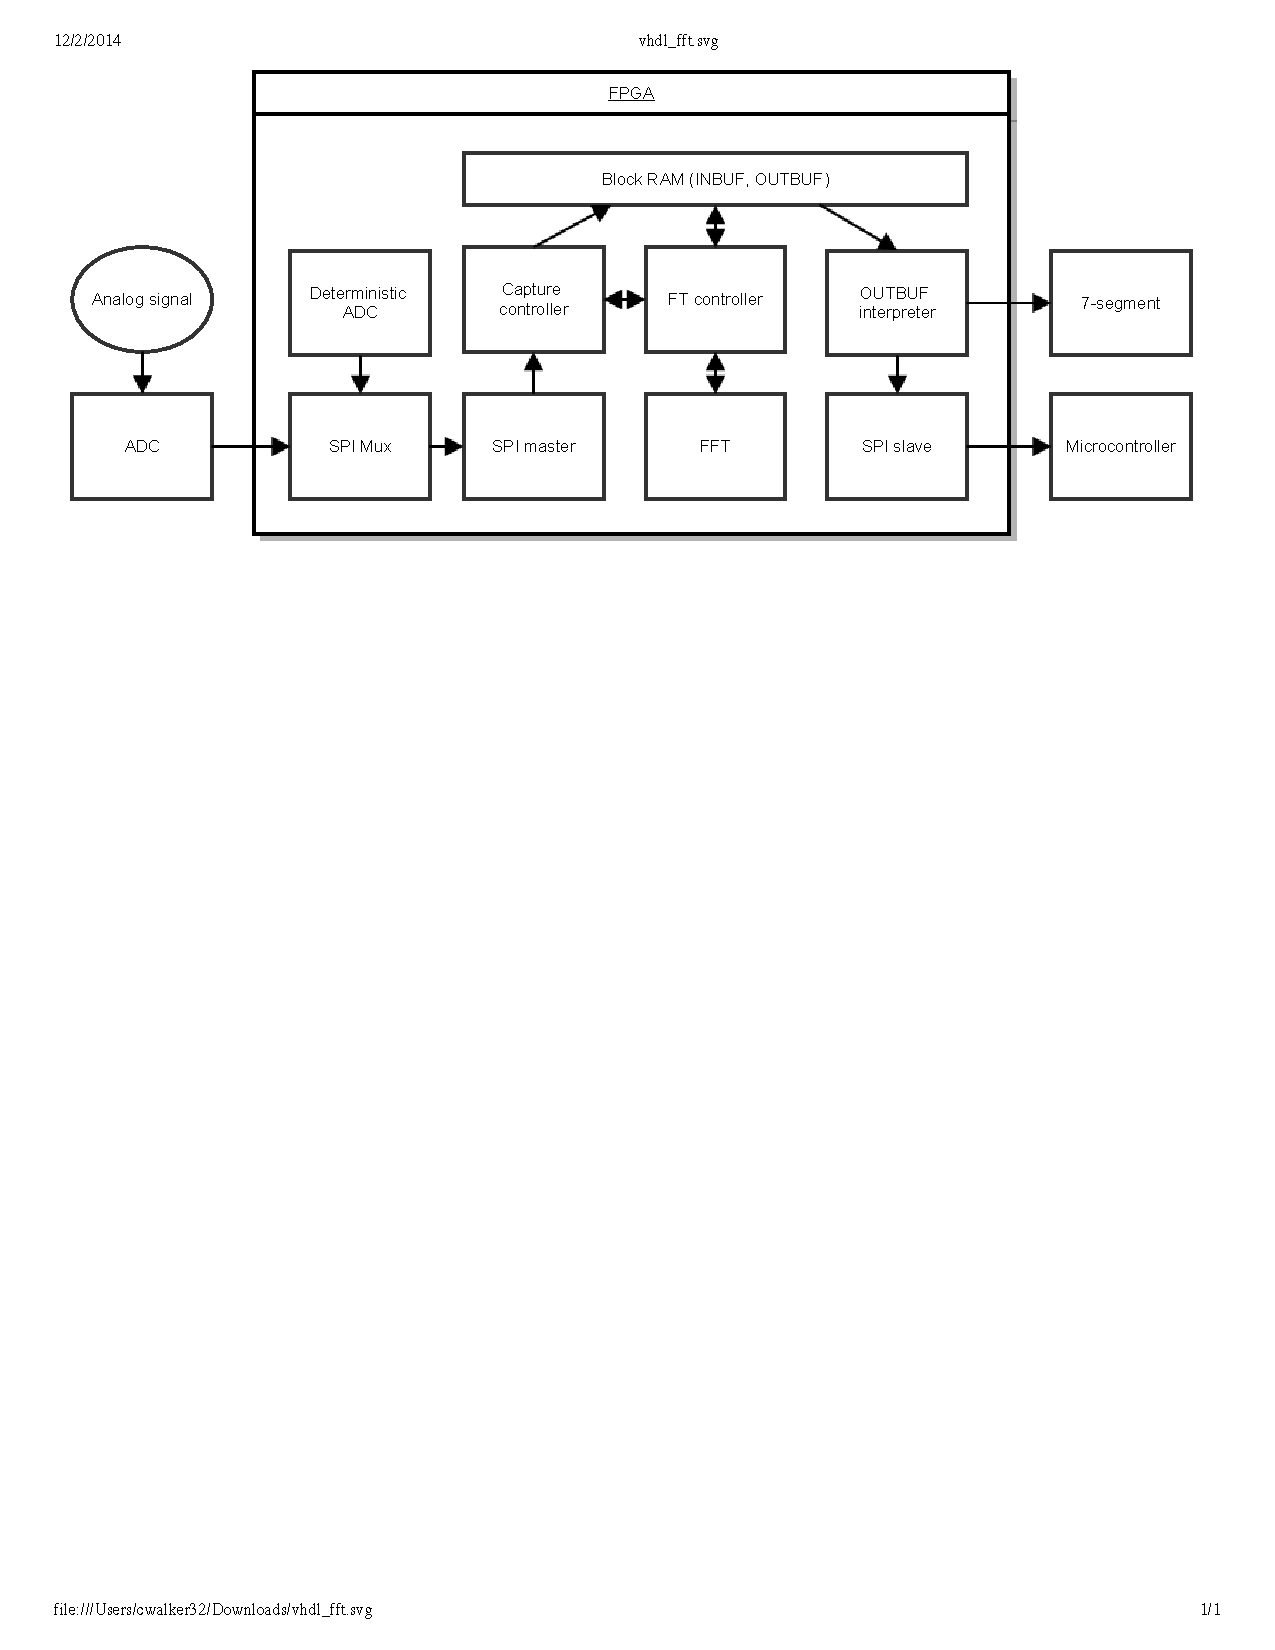
\includegraphics[trim=0 400 0 400,clip,width=140mm]{vhdl_fft.pdf}
      \caption{Block diagram of the FFT chip}
      \label{overflow}
    \end{figure}
    All of the blocks inside the FPGA device are referred to as micro-components.

    \begin{itemize}
      \item Deterministic ADC: Provides a completely predictable ADC signal to test with and substituted for a real ADC while it was shipping.
      \item SPI Mux: A simple multiplexer that selects between the external ADC and the deterministic ADC.
      \item SPI Master: An OpenCore that implements an SPI master interface. This handles the control and reading of the SPI bus from either the deterministic ADC or the external ADC.
      \item Capture Controller: This block reads samples from the SPI Master and stores the readings as complex numbers in the input buffer. The sample size is 512. It also communicates with the FT controller about when it finishes.
      \item FT controller: This block actually executes the fast Fourier transfer algorithm whenever the capture controller indicates that the input buffer is valid.
      \item Complex ALU: This block handles complex multiplications for the FT controller.
      \item OUTBUF interpreter: This block facilitates the reading of the OUTBUF by feeding words into the SPI slave module.
      \item SPI Slave: An OpenCore that implements an SPI slave interface. This handles the control and writing of the SPI bus, and it connects to an external microcontroller.
    \end{itemize}

  \section*{Simulation Results}

  \section*{Results}
    He seemed really excited about timing results so we should probably discuss this here.

  \section*{Roadblocks}

  \section*{Future Improvements}

  \section*{Conclusion}

  \clearpage
  \section*{Appendix}

  \begin{thebibliography}{9}
    \bibitem{doin}
      Doin, Jonny. \emph{SPI Master/Slave Interface.} OpenCores, 16 May 2011. Web. 13 Sept. 2014. \textless\url{http://opencores.org/project,spi_master_slave}\textgreater.
    \bibitem{reynwar}
      Reynwar, Ben. \emph{FFT on an FPGA.} FFT on an FPGA. N.p., n.d. Web. 13 Sept. 2014. \textless\url{http://www.reynwar.net/ben/docs/fft_dit/index.html}\textgreater.
    \bibitem{roberts}
      Roberts, Michael J. \emph{Signals and Systems: Analysis Using Transform Methods and MATLAB.} New York: McGraw Hill, 2012. Print.
    \bibitem{satoh}
      Satoh, Keiichi, Jubee Tada, Kenta Yamaguchi, and Yasutaka Tamura. \emph{Complex Multiplier Suited for FPGA Structure.} Computers and Communications (2008): 341-44. Web. 13 Sept. 2014.
    \bibitem{tukey}
      Wikipedia contributors. \emph{Cooley–Tukey FFT algorithm.} Wikipedia, The Free Encyclopedia. Wikipedia, The Free Encyclopedia, 27 Jun. 2014. Web. 13 Sep. 2014.
    \bibitem{dft}
      Wikipedia contributors. \emph{Discrete Fourier transform.} Wikipedia, The Free Encyclopedia. Wikipedia, The Free Encyclopedia, 2 Sep. 2014. Web. 13 Sep. 2014.
  \end{thebibliography}

\end{document}
%  \subsection*{Overview}
%    In this project we will implement the Cooley-Tukey Fast Fourier Transform algorithm on a Xilinx FPGA using VHDL.
%    The primary motivation for this is to digitally analyze musical signals, regardless of the instruments they come from.
%    Using the Cooley-Tukey algorithm, we can calculate the FFT in $O(nlog_2(n))$ time.
%    As far as implementation, the project will be split into several main components.
%    First, we will need to sample our audio for a set amount of time and store the data into a buffer in memory.
%    Then, the digital signal will need to be processed using a complex ALU.
%    Finally, the data will need to be sent to an output buffer for application specific usage.
%    This can be in the form of a 7-segment hex display (for instance if we want to print out the fundamental frequency), or a microcontroller (if we want to plot the entire sampled spectrum by passing it to a more capable platform such as Matlab).
%
%  \subsection*{Theory}
%    To understand the discrete Fourier Transform, one must first analyze its analogous continuous time form.
%    This is written most simply as
%    \begin{align*}
%    &X(\omega) = \int_{-\infty}^{\infty} x(t) e^{-j \omega t}\,dt
%    \end{align*}
%    which defines the transform of a continuous time signal $f(t)$.
%    Without getting into too many details, it defines the signal as a combination of sinusoids, making it a very useful tool for real world applications.\\
%    
%    The discrete Fourier Transform (DFT) is simply a reduction of the continuous Fourier Transform into a discrete sample space.
%    In other words, if we let $x_n$ represent a sampled version of the continuous time function $x(t)$ with a total of $N$ samples, we can replace the integral with a summation over the series, as shown below.
%    \begin{align*}
%        &X_k = \sum\limits_{n=0}^{N-1} x_n e^{\frac{-j2\pi kn}{N}}
%    \end{align*}
%    As with the continuous time case, this series gives us a glimpse into the component elements of our original signal.
%    However, it is rather costly to compute, requiring a time complexity of $O(N^2)$.
%    For each value $X_k$, a series of values from $n = 0$ to $N - 1$ must be generated and summed, using up valuable computer resources.
%    Thus, calculating the DFT in this way is very inefficient, and we must instead turn to the Fast Fourier Transform.\\
%
%    In order to perform this operation more quickly, we can utilize the Cooley-Tukey FFT algorithm.
%    However, the one requirement is that our input is strictly a power of 2.
%    That is because the algorithm works by recursively finding the FFT of smaller and smaller sample sizes of $x_n$, which arises from the fact that the transform itself is periodic.
%    The transform function can be broken into the sum of its even and odd components,
%    \begin{align*} 
%        &X_k = \sum \limits_{m=0}^{N/2-1} x_{2m}e^{-\frac{2\pi i}{N} (2m)k} + \sum \limits_{m=0}^{N/2-1} x_{2m+1} e^{-\frac{2\pi i}{N} (2m+1)k}
%    \end{align*}
%    This equation can further be simplified by making the substitutions
%    \begin{align*}
%        &E_k = \sum \limits_{m=0}^{N/2-1} x_{2m}e^{-\frac{2\pi i}{N} (2m)k}
%        &O_k = \sum \limits_{m=0}^{N/2-1} x_{2m+1} e^{-\frac{2\pi i}{N/2} mk}
%    \end{align*}
%    giving us
%    \begin{align*}
%        &X_k = E_k + e^{-\frac{2\pi i}{N} k} O_k
%    \end{align*}
%    The expression $e^{-\frac{2\pi i}{N}k}$ is commonly called the \textit{twiddle factor}.
%    Furthermore, because of the periodicity of the transform, we can calculate respective even and odd components simultaneously
%    \begin{align*}
%        &E_k = E_{k+\frac{N}{2}}
%        &O_k = O_{k+\frac{N}{2}}
%    \end{align*}
%    
%
%
%  \subsection*{In Mathematica}
%  We implemented a candidate version of the Cooley-Tukey algorithm in Mathematica. This code shows how it is possible to build a look up table of calculated results against the variables $N$ and $k$ for the calculation $e^{-\frac{2\pi i}{N} k}$. This table will not only save us time, but also complexity in the design by allowing us to simply look up this value.
%  \begin{lstlisting}
%myfasterft[x_, capn_, s_, precomputed_] := (
%   result = {};
%   If[capn == 1,
%    result = Append[result, x[[1]]],
%    result = Join[result, myfasterft[x, capn/2, 2 s, precomputed]];
%    result = 
%     Join[result, myfasterft[x[[s + 1 ;;]], capn/2, 2 s, precomputed]];
%    Do[
%     t = result[[k + 1]];
%     result[[k + 1]] = 
%      t + precomputed[[Log2[capn]]][[k + 1]]*
%        result[[k + capn/2 + 1]];
%     result[[k + capn/2 + 1]] = 
%      t - precomputed[[Log2[capn]]][[k + 1]]*
%        result[[k + capn/2 + 1]];
%     , {k, 0, capn/2 - 1}];
%    ];
%   result
%   );
%
%precomputedmatrix[datalen_] := (
%  Table[
%   Table[
%    E^(-I*2*\[Pi]*k/capn),
%    {k, 0., datalen/2 - 1}
%    ],
%   {capn, Table[2^x, {x, 1, Log2[datalen]}]}
%   ]
%  )
%
%data = Table[N[Sin[30 2 Pi n/200] + (RandomReal[] - 1/2)], {n, 512}];
%precomputed = precomputedmatrix[Length[data]];
%ListLinePlot[Abs[myfasterft[data, Length[data], 1, precomputed]], PlotRange -> All]
%  \end{lstlisting}
%  \subsection*{FPGA considerations}
%    %Describe how we plan to utilize SPI for communication, what type of logical blocks we will use and how they will work together.
%    Because we are working with a very specialized type of hardware, we must take into consideration some limiting parameters.
%    In particular, the Spartan3Es loaded on each BASYS board only have 72K RAM.
%    This means that if we want a real time FFT, we will need to optimize the space we have available, and only write to it when it is absolutely necessary.
%    We must also consider the quality of our digital input signal.
%    There are various ADC PMODs available for the BASYS boards, which range in quality from 4.8 KHz to 1 MHz in speed.
%    If we are only sampling audio, we probably won't need to gather any frequencies above 1200 Hz, so the lower end model should be fine.\\
%
%    Once our data has been collected and stored inside the FPGA, it needs to be processed.
%    This is perhaps the most challenging part of the project, as we need to implement what will be called an FTC (Fourier Transform Controller) as well as a CALU (Complex Arithmetic Logic Unit).
%    The FTC's primary function will be to keep track of the data as it moves from RAM, into the CALU, and back out into the real world.
%    This will require some heavily synchronized logic and very tight timing control to be carried out properly.
%    It will work in sync with the SPI input master to tell the CALU when data is ready to be read, and then clear the input buffer once the CALU has finished.
%    It will also need to monitor the movement of data from the output buffer into whatever output stream requires it.
%    The data may be sent directly to a microcontroller or into another component for post processing.\\
%
%    The CALU will have one primary job, which is to actually perform the FFT.
%    From its perspective, it will only the addresses of an input buffer and an output buffer, as well as a flag that tells it when to start and stop.
%    Because all of our calculations are being done inside of an FPGA, the CALU will be most composed of combinational logic at its core.
%    In theory (i.e., provided enough gates), all that needs to be built is the base case of the FFT, which takes in two numbers and outputs their sum and difference.
%    \begin{align*}
%        &y_0 = x_0 + e^{-\frac{2\pi i}{N}k}x_1
%        &y_1 = x_0 - e^{-\frac{2\pi i}{N}k}x_1
%    \end{align*}
%    This portion of the computation is commonly called a \textit{butterfly}, because the system's diagram looks vaguely like a butterfly.
%    Each of the twiddle factors included above can be calculated beforehand and stored in a lookup table for quick access before each iteration.
%    Because we will be performing the same type of computation with them each time, they are essentially constants in our system.\\
%
%  \subsection*{Block diagram}
%    Over the past few weeks we have taken what we know and outlined a basic block diagram of our device:
%    \begin{figure}[H]
%      \centering
%      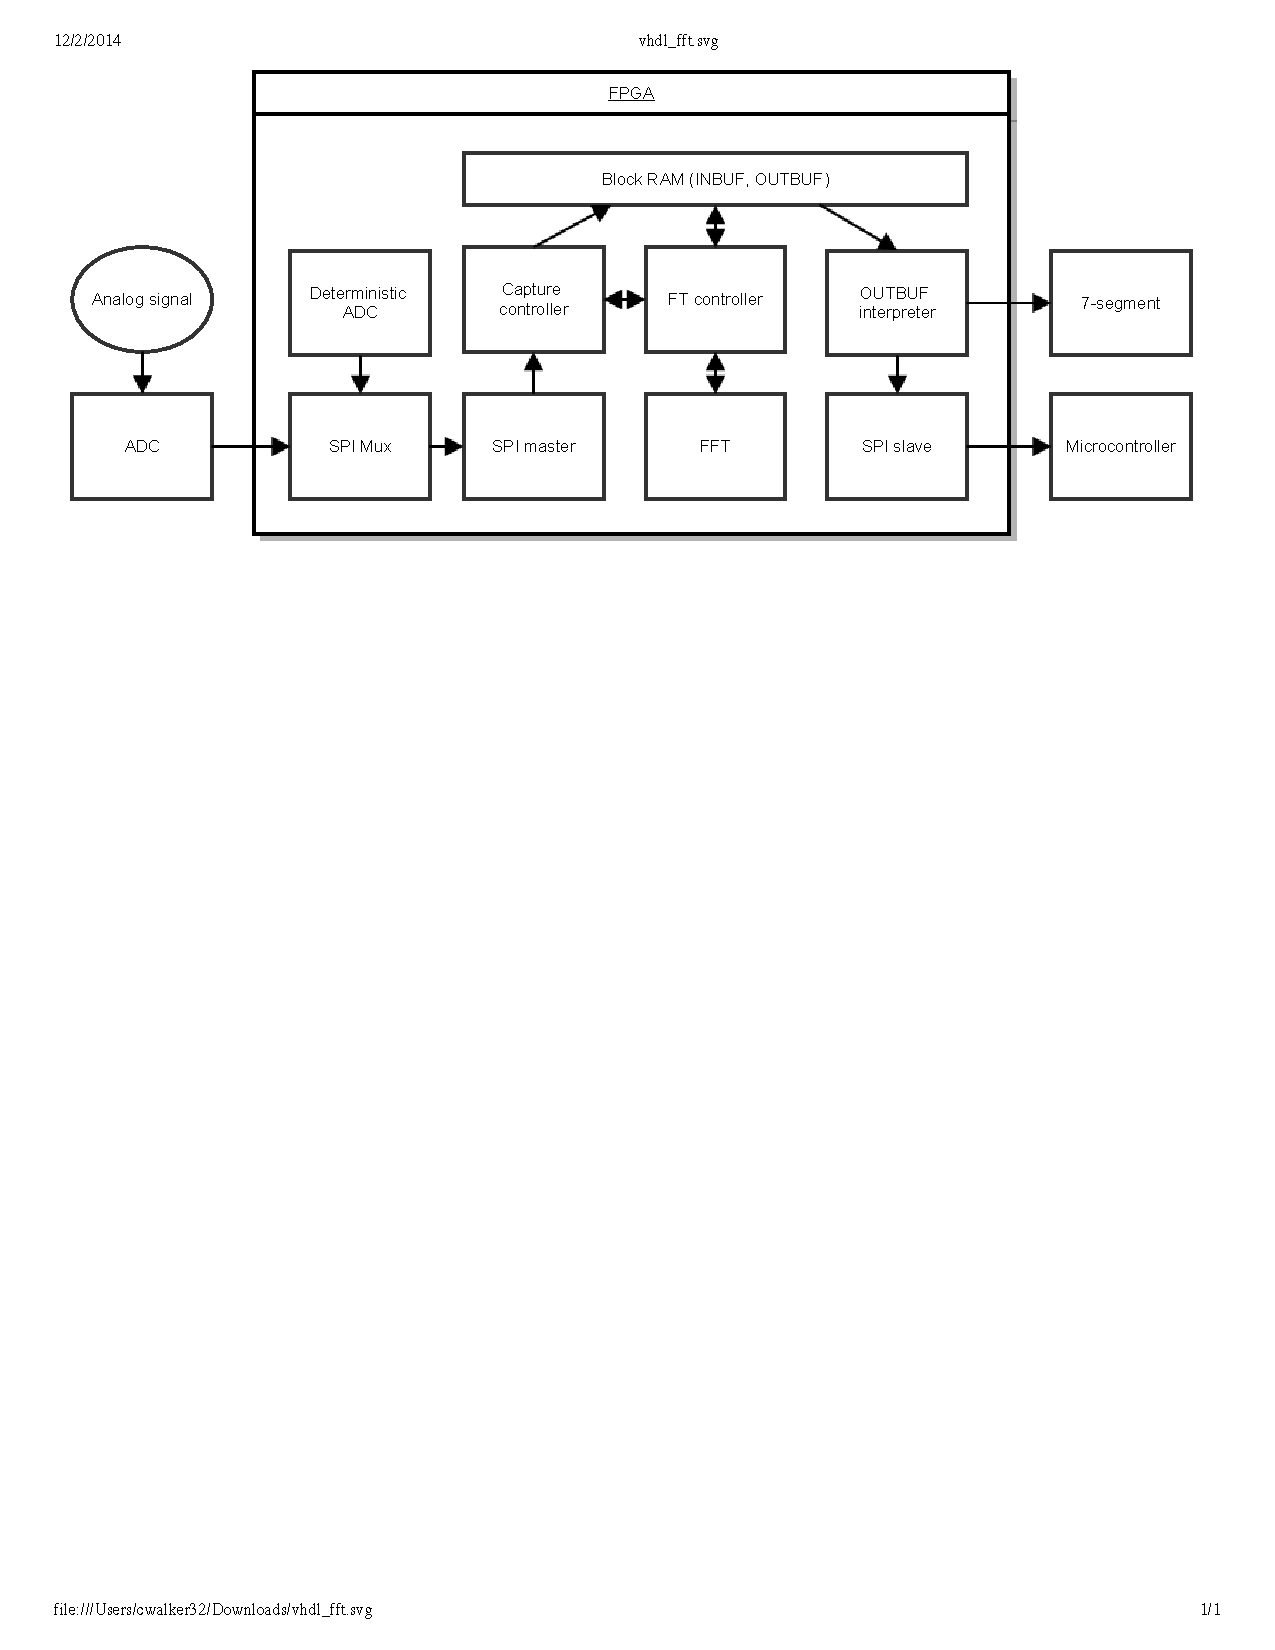
\includegraphics[trim=0 400 0 400,clip,width=140mm]{vhdl_fft.pdf}
%      \caption{Block diagram of the FFT chip}
%      \label{overflow}
%    \end{figure}
%    Now that we have divided the device into several logical blocks, we can now split up the work accordingly.
%  \subsection*{Roadmap}
%    In this section, we will describe the steps, in order, that need to be done. Our steps will essentially follow the data pipeline of the module:
%    \begin{itemize}
%      \item We will begin by implementing a deterministic "ADC" module that will emulate the interface of the real ADC but generate a fixed signal every time. We will use this signal in our own calculations so that we can then verify the outputs of the chip at each stage in the data pipeline. When we are ready to convert to real ADC signals, we can simply switch to an external ADC module using an SPI mux. This step has already been completed.
%      \item We will then implement the capture controller. This controller will have an SPI master unit that can read from the ADC. It will be also connected to the block RAM to write the input buffer.
%      \item Next, we will work on the heart of the chip, the FT controller. This controller will first simply implement the DFT algorithm. It will utilize the complex number ALU to make calculations.
%      \item After the FT controller, we will implement an OUTBUF interpreter that is responsible for outputting the results of the FT controller to the rest of the world using SPI.
%      \item Once all of this is done, we will finish converting our FT controller from using the simple DFT algorithm to the more complex Cooley-Tukey FFT algorithm.
%      \item If we have further time still, we will build interesting demonstrations of this device.
%    \end{itemize}
%  \subsection*{Resources}
%    While our aim is to implement the entire Fast Fourier Transform with our own code, there are some blocks of our design that are common practice to reuse. Those blocks are the SPI modules. While SPI is not a complicated communication protocol, it requires a fair amount of time to implement. There is a great resource online called OpenCores. This resource is essentially a collection of open source HDL modules that can be freely used in designs. We will be using the "SPI Master/Slave Interface" module a few times in our design to implement SPI.
%  \subsection*{Possible extensions}
%    The Fast Fourier Transform algorithm applied to an arbitrary voltage signal is very useful. Because our final chip will provide such capability, we have the option of using our newly-designed chip with multiple different applications. \\
%  
%    One of our ideas is to attach a microphone and a preamp and use the frequency-domain signal to determine the musical note being played. We could also build a tuner for a guitar. \\
%    
%    Additionally, we could connect an audio signal directly from any music player and display a graphic equalizer effect using either a computer or microcontroller that will interface with our chip. \\
%
%    Finally, provided we are able to tune our chip and ADC to operate fast enough, we might be able to build a radio wave analyzer for very long wavelength signals. This device would almost certainly be too slow for any serious RF work, but it would still be an interesting extension. \\
%
%    These extensions are not crucial to our design but might serve as a great demonstration when we present the device to the class.
